\section{Teoremas de Desargues, Pappus, Pascal}

Obs: Las soluciones en esta parte en especial est\'an escritas de manera que el orden de las letras determina la forma en que se usar\'a el teorema, es por eso que no se brindan muchos detalles
\begin{sol}
	Para la primera apliquemos el teorema de Pappus en los puntos $\{A, F, D\}$ y $\{B, E, C\}$. Para la segunda parte utilice el teorema de Desargues en los tri\'angulos $\triangle BED$ y $\triangle AFC$.
\end{sol}

\begin{sol}
	Utilice el teorema de Desargues en los tri\'angulos $\triangle ABC$ y $\triangle A'B'C'$. 
\end{sol}

\begin{sol}
	Utilice el teorema de Pappus en los puntos $A_{1}, B_{1}, C_{1}$ y $A_{2}, B_{2}, C_{2}$. 
\end{sol}

\begin{sol}
	Sea $Q =BA \cap CD$, $P = BC \cap AD$. Sea $M$ el punto medio de $BC$ y $N$ el punto medio de $AB$. Por el teorema de Pappus en los puntos $M, C, P $ y $N, A, Q$ tenemos que $PN\cap QM, CN \cap AM y D$ son colineales. Pero como $\triangle BCQ$ y $\triangle BAP$ son is\'oceles, tenemos que $G = CN \cap AM$, y $ O = PN \cap QM$. Lo que completa la prueba.
\end{sol}

\begin{sol}
	Probaremos que el incentro $I$ del tri\'angulo $\triangle ABC$ pertenece a todos los segmentos mencionados (aqui solo ser\'a probado un caso, puesto que el resto de los casos son an\'alogos). Use el teorema de Pascal en los conjuntos de puntos $\{C', A, B'\}$ y $\{B, A', C\}$. Observe que los puntos determinados por el teorema de Pascal son $I$ $(= BB' \cap CC')$, $Q$ y $T$. Por lo que $I\in QT$ y el resultado sigue.
\end{sol}

\begin{sol}
	Use el teorema de Brianchon admitiendo puntos colineales en el hex\'agono.
\end{sol}


\begin{sol}
	Primeramente, veamos que $X = ME\cap NF$, $Y = NQ \cap PM$ y $B$ son colineales. Para eso, use el teorema de Pascal con los conjuntos de puntos $\{N, P, E\}$ y $\{M, A, F\}$. Los puntos de intersecci\'on que el teorema brinda son exactamente $B, X$ e $Y$. Sabemos por el ejercicio anterior que $Y\in BD$, por lo que el resultado sigue.
\end{sol}

\begin{sol}
	Literalmente un corolario del ejercicio anterior. 
\end{sol}

\begin{sol}
	Soluci\'on pendiente :(
	\begin{figure}[h!]
		\centering
		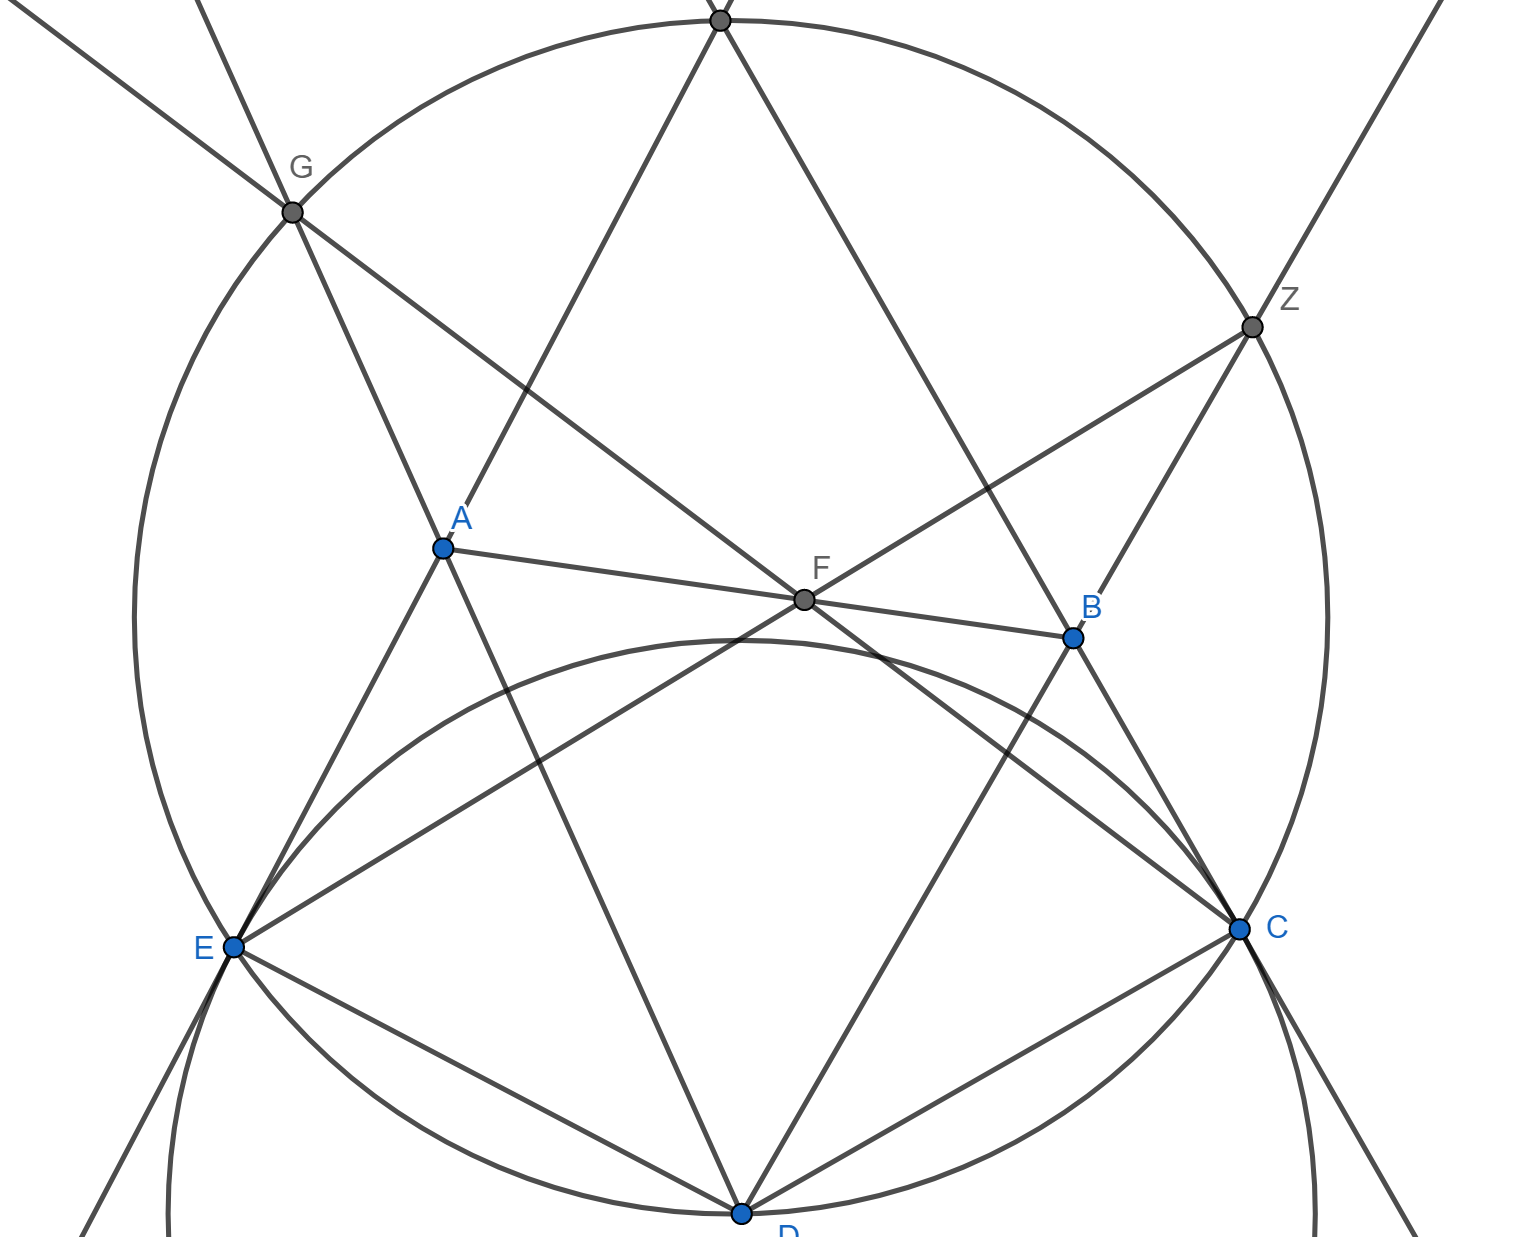
\includegraphics[scale=0.2]{Imgs/JT4.png}
	\end{figure}
\end{sol}

\begin{sol}
	Utilice Ceva trigonom\'etrico (Usando que $\angle HAC = \angle HBC$, por ejemplo)
	
\end{sol}